% Options for packages loaded elsewhere
\PassOptionsToPackage{unicode}{hyperref}
\PassOptionsToPackage{hyphens}{url}
%
\documentclass[
  a4paper,
  twoside, 11pt]{article}
\usepackage{lmodern}
\usepackage{amssymb,amsmath}
\usepackage{ifxetex,ifluatex}
\ifnum 0\ifxetex 1\fi\ifluatex 1\fi=0 % if pdftex
  \usepackage[T1]{fontenc}
  \usepackage[utf8]{inputenc}
  \usepackage{textcomp} % provide euro and other symbols
\else % if luatex or xetex
  \usepackage{unicode-math}
  \defaultfontfeatures{Scale=MatchLowercase}
  \defaultfontfeatures[\rmfamily]{Ligatures=TeX,Scale=1}
\fi
% Use upquote if available, for straight quotes in verbatim environments
\IfFileExists{upquote.sty}{\usepackage{upquote}}{}
\IfFileExists{microtype.sty}{% use microtype if available
  \usepackage[]{microtype}
  \UseMicrotypeSet[protrusion]{basicmath} % disable protrusion for tt fonts
}{}
\makeatletter
\@ifundefined{KOMAClassName}{% if non-KOMA class
  \IfFileExists{parskip.sty}{%
    \usepackage{parskip}
  }{% else
    \setlength{\parindent}{0pt}
    \setlength{\parskip}{6pt plus 2pt minus 1pt}}
}{% if KOMA class
  \KOMAoptions{parskip=half}}
\makeatother
\usepackage{xcolor}
\IfFileExists{xurl.sty}{\usepackage{xurl}}{} % add URL line breaks if available
\IfFileExists{bookmark.sty}{\usepackage{bookmark}}{\usepackage{hyperref}}
\hypersetup{
  hidelinks,
  pdfcreator={LaTeX via pandoc}}
\urlstyle{same} % disable monospaced font for URLs
\usepackage[top=2cm, outer=3.5cm, bottom=3cm, inner=3.5cm]{geometry}
\usepackage{longtable,booktabs}
% Correct order of tables after \paragraph or \subparagraph
\usepackage{etoolbox}
\makeatletter
\patchcmd\longtable{\par}{\if@noskipsec\mbox{}\fi\par}{}{}
\makeatother
% Allow footnotes in longtable head/foot
\IfFileExists{footnotehyper.sty}{\usepackage{footnotehyper}}{\usepackage{footnote}}
\makesavenoteenv{longtable}
\usepackage{graphicx,grffile}
\makeatletter
\def\maxwidth{\ifdim\Gin@nat@width>\linewidth\linewidth\else\Gin@nat@width\fi}
\def\maxheight{\ifdim\Gin@nat@height>\textheight\textheight\else\Gin@nat@height\fi}
\makeatother
% Scale images if necessary, so that they will not overflow the page
% margins by default, and it is still possible to overwrite the defaults
% using explicit options in \includegraphics[width, height, ...]{}
\setkeys{Gin}{width=\maxwidth,height=\maxheight,keepaspectratio}
% Set default figure placement to htbp
\makeatletter
\def\fps@figure{htbp}
\makeatother
\setlength{\emergencystretch}{3em} % prevent overfull lines
\providecommand{\tightlist}{%
  \setlength{\itemsep}{0pt}\setlength{\parskip}{0pt}}
\setcounter{secnumdepth}{-\maxdimen} % remove section numbering
% change line spacing
\usepackage[onehalfspacing]{setspace}

% change font to Helvetica for titles and Garamond for body text
\usepackage[scaled]{helvet}
\usepackage{garamondx}
\usepackage[T1]{fontenc}
% \renewcommand\familydefault{\sfdefault}

% allow coloured text and boxes
\usepackage{xcolor}
\definecolor{uclyellow}{HTML}{F6BE00}

% change section titles
\usepackage{titlesec}
\titleformat{\section}{\bigskip\raggedright\LARGE\sffamily}{\thesection}{0.5em}{}[\titlerule]

% allow absolute positioning of blocks on title page
\usepackage[absolute]{textpos}
\setlength{\TPHorizModule}{1cm}
\setlength{\TPVertModule}{\TPHorizModule}
\textblockorigin{0cm}{0cm}

% override default placement of figures by pandoc, which is different from the latex default
% this code works in conjunction wit the knitr option `fig.pos = 'tbp'`
\usepackage{float}

% move captions above figures
% \usepackage{floatrow}
% \floatsetup[figure]{capposition=top}

% make tables prettier
\usepackage{booktabs}

% prevent widows and orphans
% \widowpenalty 10000
% \clubpenalty 10000

% setup PDF options
\hypersetup{
    colorlinks=true,
    linkcolor=blue,
    filecolor=blue,      
    urlcolor=blue,
    pdftitle={Stop and search in London},
    bookmarks=true
}

\author{}
\date{\vspace{-2.5em}}

\begin{document}

\frenchspacing

\raggedright

\raggedbottom

\begin{textblock*}{21cm}(0mm, 0mm)
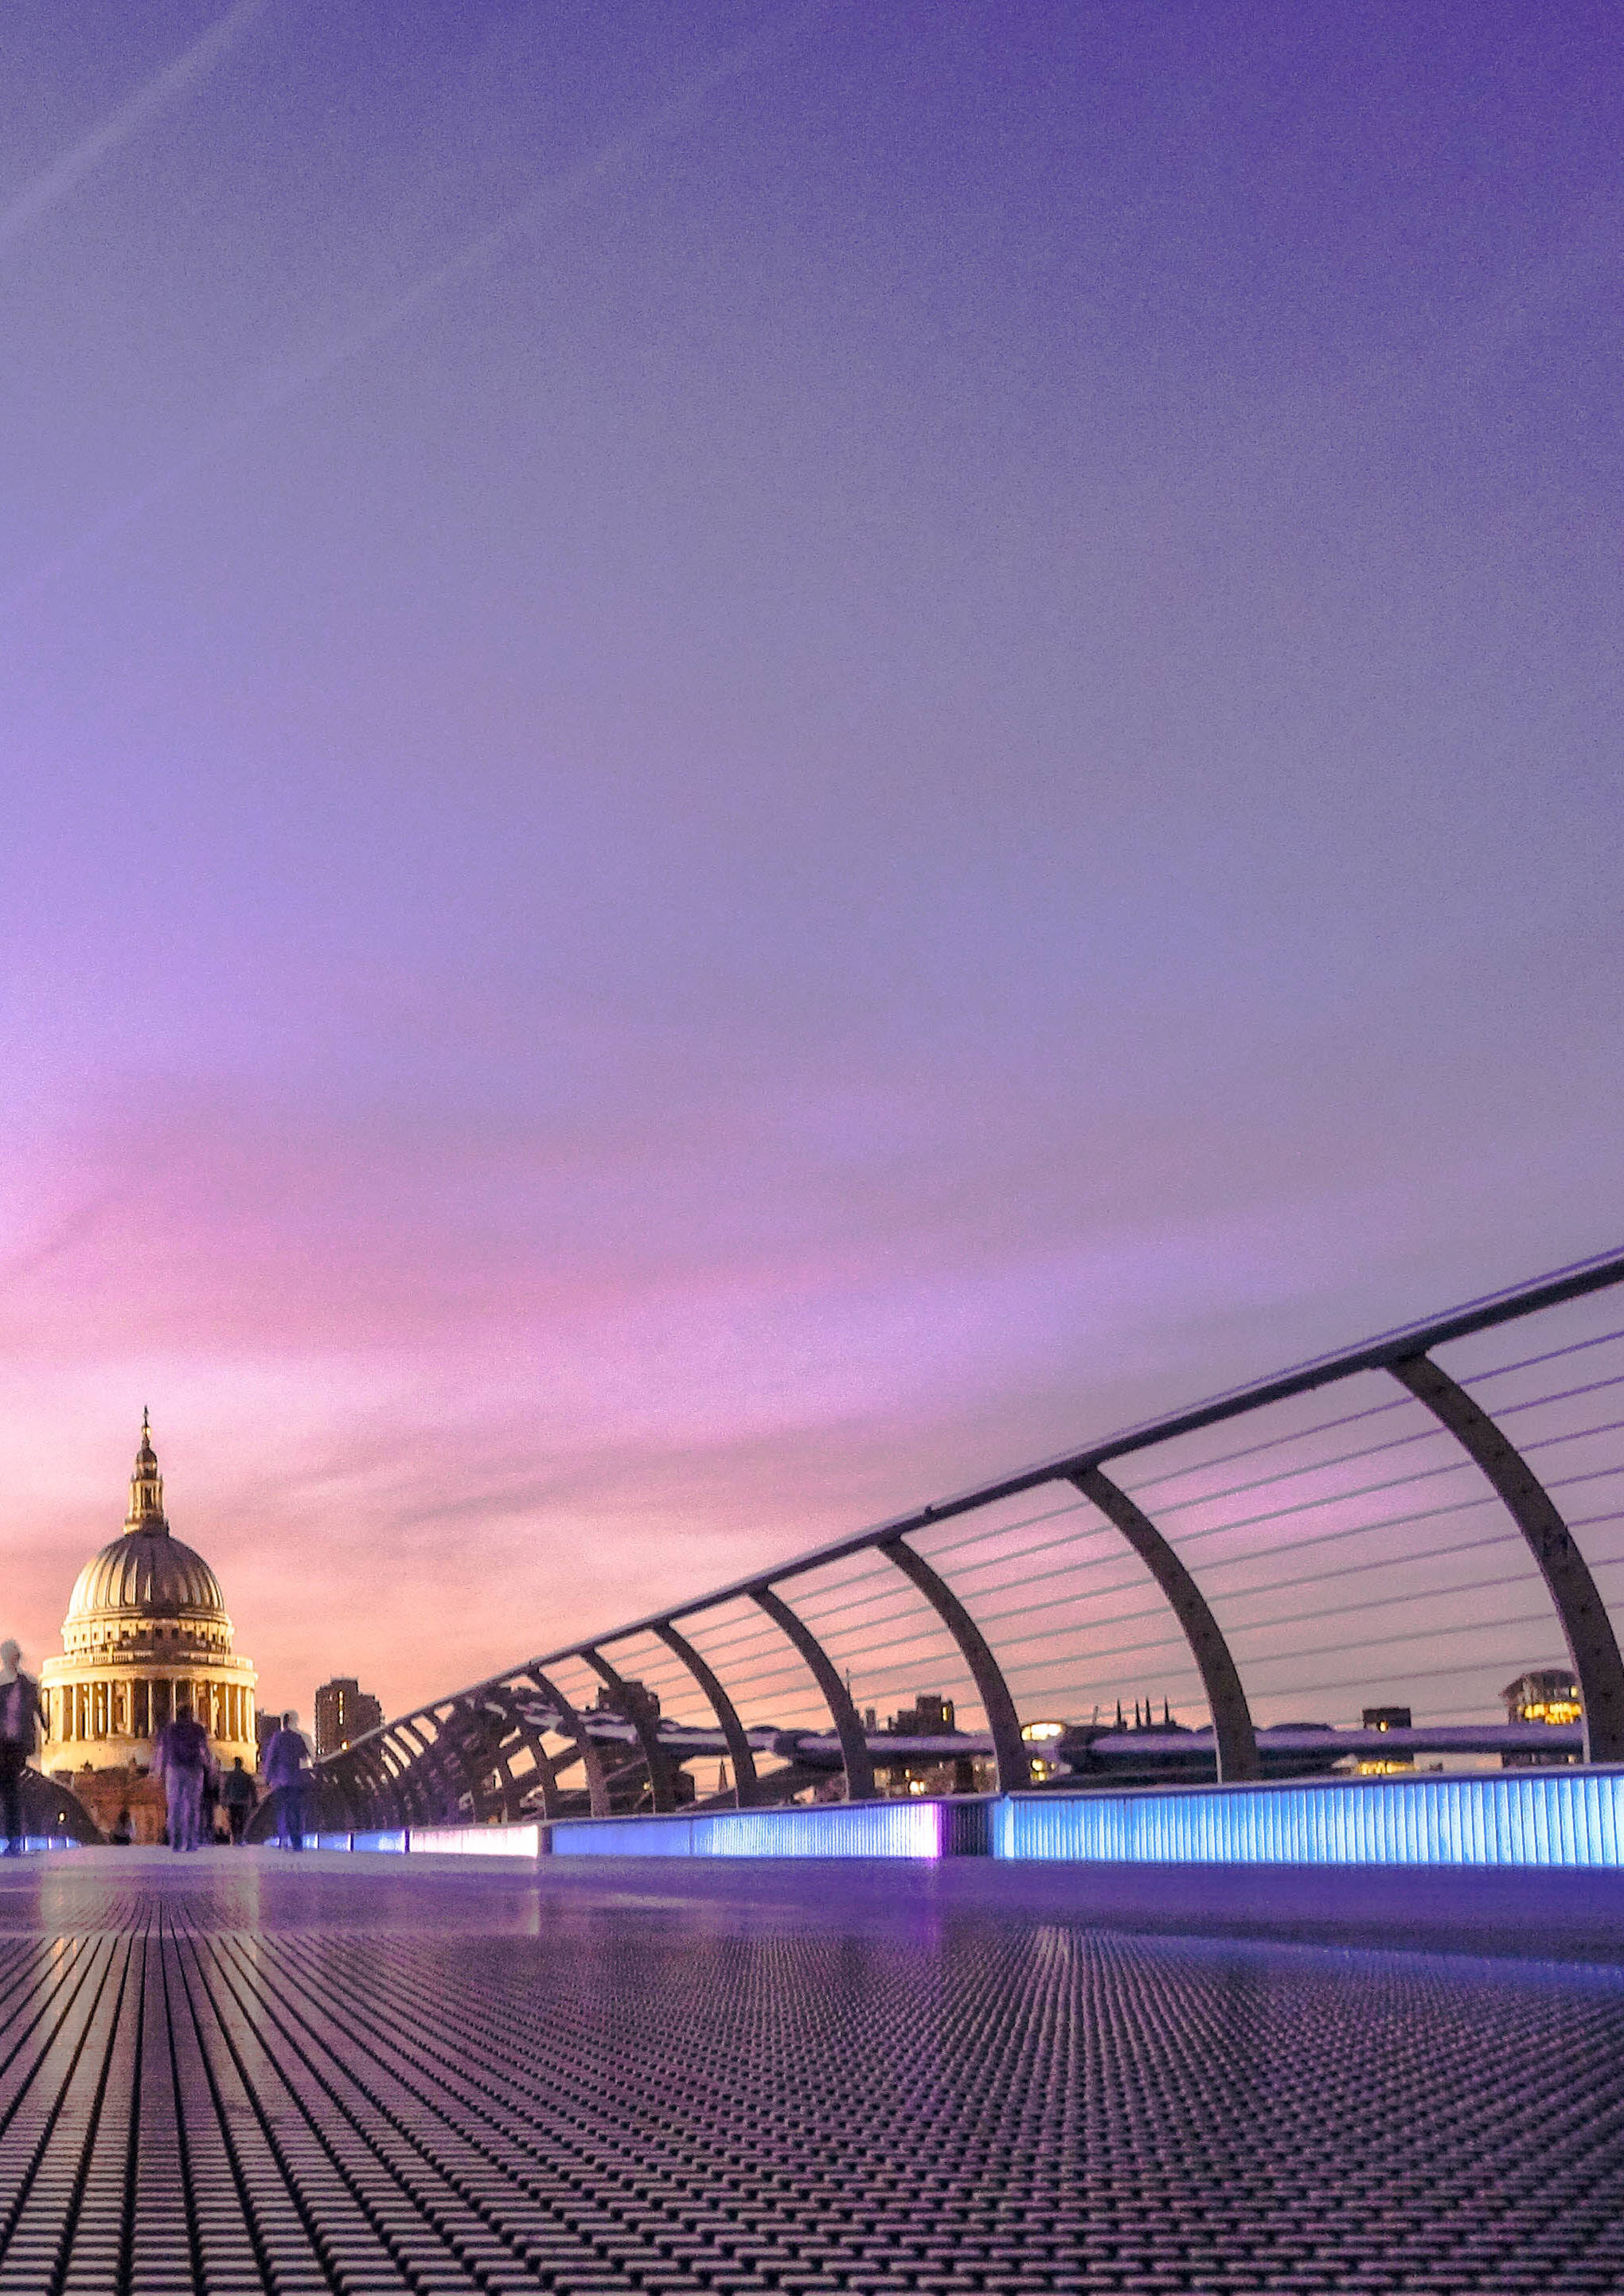
\includegraphics[width=21cm,height=29.7cm]{cover_image_2020_q3.jpg}
\end{textblock*}

\begin{textblock*}{21cm}(0mm, 0mm)

\includegraphics[width=21cm]{ucl-banner-port-yellow-rgb-lg.png}
\end{textblock*}

\begin{textblock*}{21cm}(1cm,1cm)
\textbf{\sffamily INSTITUTE FOR GLOBAL CITY POLICING}
\end{textblock*}

\begin{textblock*}{18cm}(3cm, 13.66cm)
\raggedright \sffamily
\begin{singlespace}
\colorbox{white}{\hspace{1cm}\parbox[c][5.9cm]{16cm}{
{\fontsize{40}{32}\selectfont \bfseries \mbox{Stop and search}\\\mbox{in London}
\vspace{6pt}}

{\fontsize{40}{32}\selectfont \mbox{July to September 2020} }

}\hspace{1cm}}
\end{singlespace}
\end{textblock*}

\begin{textblock*}{11.43cm}(0cm, 24.13cm)
\colorbox{uclyellow}{\parbox[c][2.63cm]{\textwidth}{
\centering \bfseries \sffamily \fontsize{16}{16}\selectfont 
Dr Matt Ashby\ \ |\ \ November 2020
}}
\end{textblock*}

~

\thispagestyle{empty}
\newpage

\hypertarget{main-points}{%
\section{Main points}\label{main-points}}

\textbf{\sffamily Police in London stopped and searched 67,997 people and vehicles in the three months from July to September 2020. The number of searches has generally increased over the past two years.}

\textbf{\sffamily 65\% of searches were for drugs, with 76\% of all searches resulting in no further action.}

\textbf{\sffamily Searches are heavily concentrated in some areas -- half of all searches occurred in 9\% of neighbourhoods.}

\hypertarget{introduction}{%
\section{Introduction}\label{introduction}}

Stop and search is a legal power that allows police officers to search people to find out if they are carrying prohibited items such as drugs, weapons or stolen goods. Stop and search means officers can confirm if a person is or is not in possession of contraband without arresting them and taking them to a police station, but it is also a source of tension between police and communities. \href{https://whatworks.college.police.uk/Research/Documents/SS_and_crime_report.pdf}{A review by the College of Policing} found little relationship between how many searches police do and how much crime occurs, but \href{https://www.met.police.uk/advice/advice-and-information/st-s/stop-and-search/why-we-use-stop-and-search/}{police insist stop and search helps them fight crime}. This report is the first of a series that will analyse stop and search in London each quarter.



\begin{figure}[bh]

{\centering 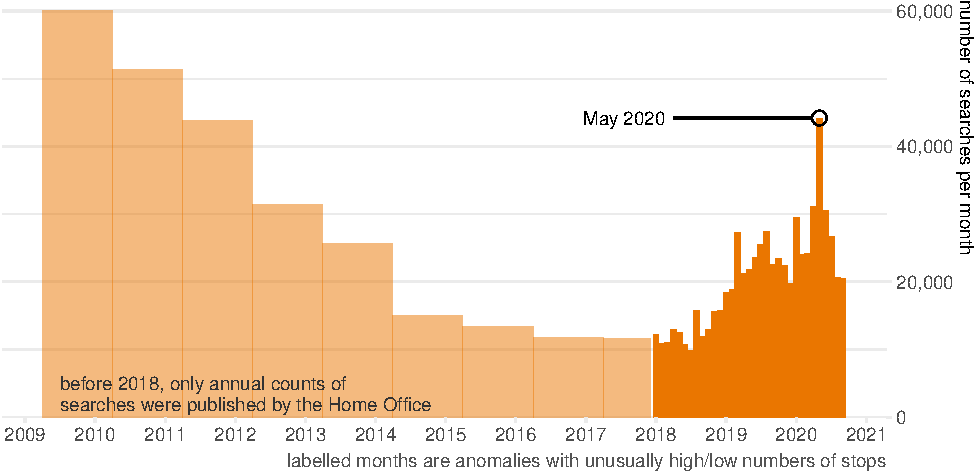
\includegraphics{2020-Q3_files/figure-latex/chart-trend-overall-1} 

}

\caption{Number of stop-and-searches in London, January 2018 to September 2020}\label{fig:chart-trend-overall}
\end{figure}

\textbf{Between July and September 2020, police officers in London carried out 67,997 stop-and-searches}, or about 5,231 per week. Of those, 97\% were conducted by the Metropolitan Police, 2\% by British Transport Police and 1\% by City of London Police. Across the three forces, 75\% of stops were of pedestrians, 23\% of people in vehicles and 2\% of only vehicles.

The number of searches carried out in July to September 2020 was \textbf{a decrease of 36\% from the previous quarter} and the largest quarterly change since at least the first quarter of 2018 (Figure \ref{fig:chart-trend-overall}).
This decrease was contrary to the upward trend since 2018, with stops having \textbf{increased by 4\% per month on average over the past two years.} Prior to 2018, the number of searches had decreased every year since 2009, dropping by 81\% in nine years.

\hypertarget{what-items-are-people-searched-for}{%
\section{What items are people searched for?}\label{what-items-are-people-searched-for}}



\begin{figure}[tb]

{\centering 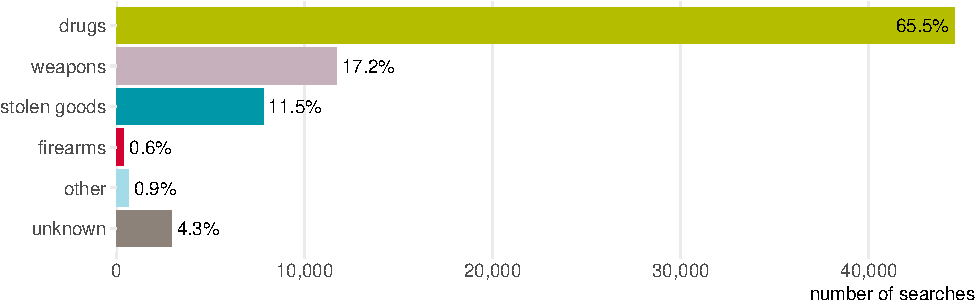
\includegraphics{2020-Q3_files/figure-latex/chart-search-types-1} 

}

\caption{Searches by type of object being searched for, July to September 2020}\label{fig:chart-search-types}
\end{figure}

Police officers are empowered to search people for different items -- including drugs, items to use in theft or criminal damage, stolen goods, weapons and even some fireworks -- under different acts of parliament. Although police emphasise that stop and search ``\href{https://www.met.police.uk/police-forces/metropolitan-police/areas/about-us/about-the-met/stop-and-search/}{protects Londoners by taking weapons off the streets}'', only about one in six searches between July and September 2020 were for weapons -- \textbf{65\% of searches were for drugs} (Figure \ref{fig:chart-search-types}).



\begin{figure}[bh]

{\centering 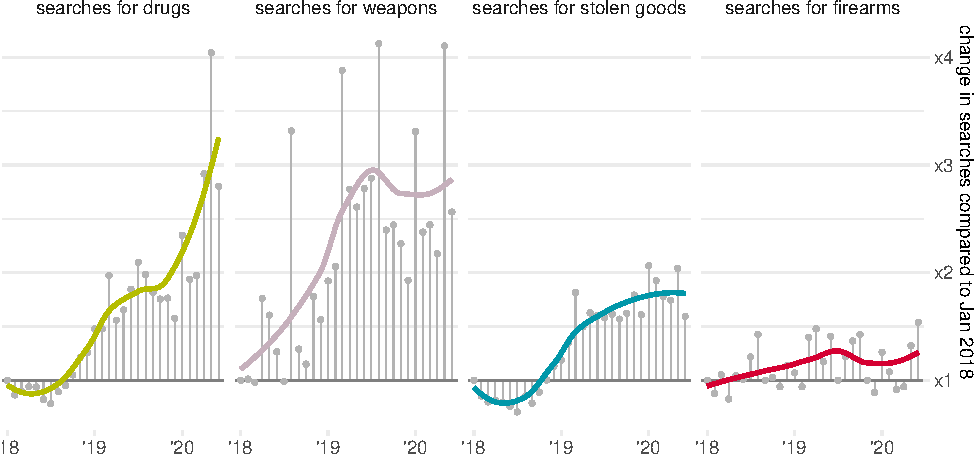
\includegraphics{2020-Q3_files/figure-latex/chart-search-types-change-1} 

}

\caption{Change in number of searches by type, January 2018 to September 2020}\label{fig:chart-search-types-change}
\end{figure}

About 95\% of searches are looking for the four main types of contraband: drugs, firearms, stolen goods and weapons. Since 2018, the number of searches for all these items have remained largely static (Figure \ref{fig:chart-search-types-change}).

Police can search people for weapons using two different legal powers. Searches under \href{https://www.legislation.gov.uk/ukpga/1984/60/section/1}{section 1 of the Police and Criminal Evidence Act 1984} (PACE) require the officer to have ``reasonable grounds for suspecting'' that the person is carrying an offensive weapon or other prohibited item. Conversely, officers can search people under \href{https://www.legislation.gov.uk/ukpga/1994/33/section/60}{section 60 of the Criminal Justice and Public Order Act 1994} (CJPOA) without having any reason to think the person has a weapon, as long as a more-senior officer believes ``incidents involving serious violence may take place'' in the area. These `section 60' searches are particularly controversial because they allow officers to search \emph{anyone} in an area, even if there is no reason to think they have a weapon in their possession. Between July and September 2020, 92\% of weapons searches are based on reasonable suspicion under PACE section 1, with the remaining 8\% based on authorisations under CJPOA section 60. Police do not publish any information about authorisations made under section 60, so it is difficult to track any patterns or trends.



\begin{figure}[tb]

{\centering 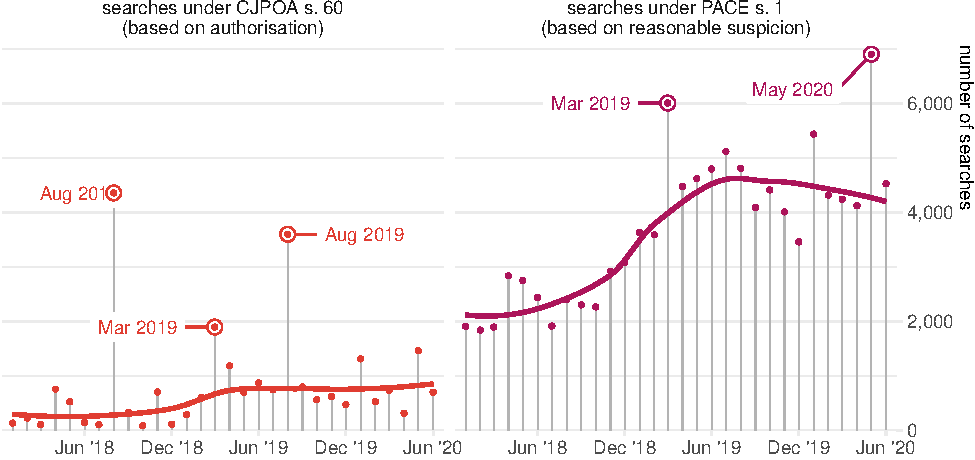
\includegraphics{2020-Q3_files/figure-latex/chart-trend-weapons-1} 

}

\caption{Change in number of searches for weapons, January 2018 to September 2020}\label{fig:chart-trend-weapons}
\end{figure}

Searches based on reasonable suspicion the person being searched is carrying a weapon have remained largely static over the past two years (Figure \ref{fig:chart-trend-weapons}). In comparison to that trend, the number of these searches in the third quarter of 2020 was within the expected range -- prior to this quarter, PACE section 1 searches had been anomalously high in March 2019 and May 2020.
No-suspicion searches under section 60 have remained largely static over the past two years, with the number of these searches between July and September 2020 within the range that would be expected based on that trend. Before that, section 60 searches had been anomalously high in August 2018 and August 2019. The number of searches under section 60 is often higher in August because of searches associated with the Notting Hill Carnival.

\hypertarget{who-do-police-search}{%
\section{Who do police search?}\label{who-do-police-search}}

Of the 66,894 searches of pedestrians and vehicle occupants from July to September 2020, \textbf{92\% were searches of men or boys}. Of all people searched, 16\% were aged under 18, 38\% were between 18 and 24, and 45\% were 25 or older. The self-defined ethnicity of the person searched was known for 77\% of searches, of which 42\% of people described themselves as white, 32\% as Black/Black British and 18\% as Asian/Asian British.

\textbf{Search rates vary hugely across different groups}. Of the 32 combinations of sex, age and self-defined ethnicity present in the search data, 13 groups were searched at a higher rate than the rate for the population as a whole (Figure \ref{fig:chart-disparity}). While disparity between ethnic groups has generated much comment, being male and being aged under 35 are more-powerful predictors of a group having a higher search rate than that group being non-white. The reasons for these differences are likely to be complex: many types of offending are concentrated among some groups (particularly young men) as well as in some neighbourhoods, and there are \href{https://www.bbc.co.uk/news/uk-47300343}{longstanding issues of bias and stereotyping among police and in society}. There is also an interaction between factors such as deprivation and the amount of time people spend in public (where almost-all searches occur). There is no way to know from the data analysed here what combination of these factors drives the disparities in search rates.



\begin{figure}[tb]

{\centering 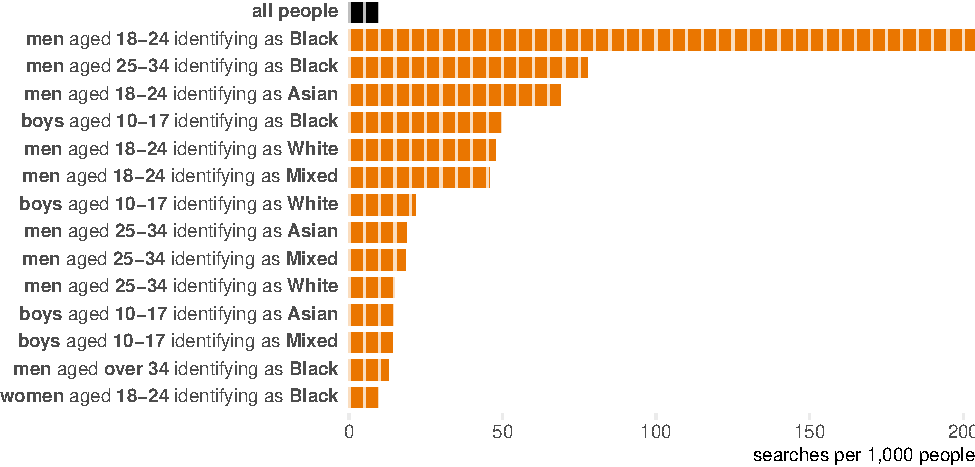
\includegraphics{2020-Q3_files/figure-latex/chart-disparity-1} 

}

\caption{Search rates for different demographic groups, July to September 2020}\label{fig:chart-disparity}
\end{figure}

In comparison to the population as a whole, people in the group with the highest search rate (men aged 18-24 identifying as Black) are on-average 19 times more likely to be stopped and searched. Disparities in search rates also vary according to the type of search. Disparity is highest in searches for weapons (based on reasonable suspicion), for which men aged 18-24 identifying as Black were 29 times more likely to be searched than the population at large. Of the 32 combinations of age, ethnic-group and sex categories present in the data, the rate of searches was highest for all five of the main types of search for men aged 18-24 who identified as Black. It is important to note that these disparity ratios only represent \emph{average} search rates for different groups -- they do not reflect the individual experience of everyone in each group. It is likely that a small number of people in each group are being searched repeatedly while others are searched far less often, but since police do not publish data on repeated searches it is difficult to know how this affects overall search rates.

\hypertarget{how-often-do-police-find-items-during-searches}{%
\section{How often do police find items during searches?}\label{how-often-do-police-find-items-during-searches}}

The purpose of stop and search is to ``enable officers to allay or confirm suspicions about individuals without exercising their power of arrest'' (\href{https://www.gov.uk/guidance/police-and-criminal-evidence-act-1984-pace-codes-of-practice}{PACE Code A, paragraph 1.4}). As such, a search that does not find what is being searched for can be considered successful if it prevents an innocent person being arrested and a police officer being taken off the street unnecessarily. As such, there is not necessarily an optimal proportion of searches that should result in the officer finding what they are looking for. Measuring outcomes is also difficult: officers may have legitimate grounds to search a group of people (e.g.~all the occupants in a vehicle believed to contain a firearm) when only one person has contraband in their possession. Nevertheless, all searches are an ``intrusion on the liberty of the person'' (PACE Code A, paragraph 1.2) and high proportions of searches that do not find anything may indicate that searches are not well targeted.

The data released by the Home Office do not specify whether or not the item police were looking for was found during a search. Instead, we can measure whether a search resulted in some formal criminal-justice process. This is not a perfect measure of whether an item was found during a search, because a person might be arrested for some other reason (for example because there was an outstanding warrant for their arrest) or contraband might be found but police deal with it informally. Nevertheless, this is the least-worst measure of search outcomes that is currently available.



\begin{figure}[tb]

{\centering 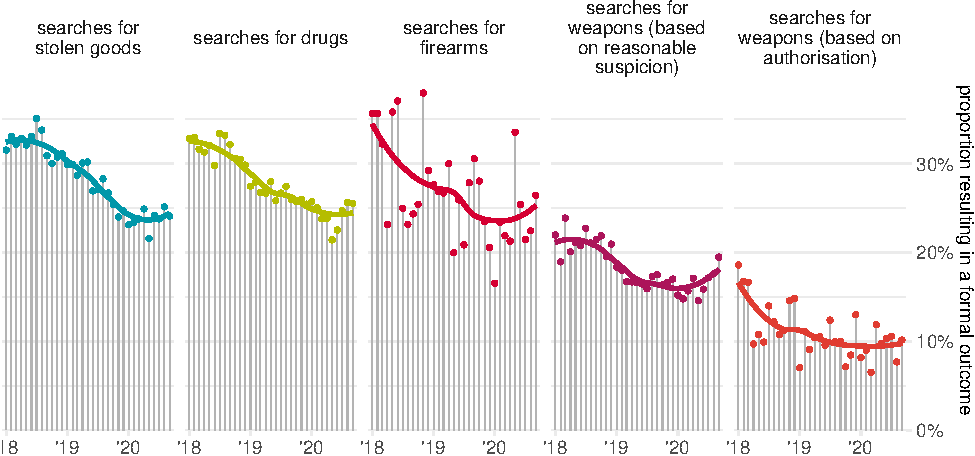
\includegraphics{2020-Q3_files/figure-latex/chart-results-1} 

}

\caption{Change in proportion of searches with a formal outcome, January 2018 to September 2020}\label{fig:chart-results}
\end{figure}

Overall, about 24\% of searches in the third quarter of 2020 resulted in a formal criminal-justice outcome (arrest, charge by post, caution, fixed penalty, community/local resolution or drugs warning), while the remaining \textbf{76\% of searches resulted in no further action.} Over the past two years, searches for stolen goods have been most likely to lead to a formal outcome, while 90\% of searches for weapons under a section 60 authorisation resulted in no further action.

In the past two years, the proportion of searches for drugs, stolen goods and weapons (based on reasonable suspicion) resulting in a formal outcome have all decreased (Figure \ref{fig:chart-results}). Overall, \textbf{the proportion of stops with a formal outcome has dropped from 28\% in 2018 to 22\% in the past 6 months}.

When a stop does result in formal action, the most common outcome is arrest (used in 53\% of cases with a formal outcome). However, which action police choose varies with the type of search: 88\% of positive searches for firearms result in arrest, compared to only 39\% of positive searches for drugs. The outcomes of some searches suggest that the outcome does not relate to the type of contraband that police were looking for. For example, fixed penalties are not a legally available option for dealing with weapons or firearms offences, but 6\% of formal outcomes to searches for weapons based on reasonable suspicion, 15\% of formal outcomes to searches for weapons based on section-60 authorisations and 3\% of formal outcomes to searches for firearms were fixed penalties. This suggests that some weapons and firearms searches result in police not finding weapons but discovering more-minor offences such as cannabis possession.

While the rate of searches varies between ethnic groups, the probability of a search resulting in a formal criminal-justice outcome is broadly the same across ethnicities -- over the past six months, the probability of a formal outcome to searches of Black or Asian people was not significantly different from the probabilty of a formal outcome to searches of White people for any of the main search types (Figure \ref{fig:chart-outcomes-ethnicity}).



\begin{figure}[tb]

{\centering 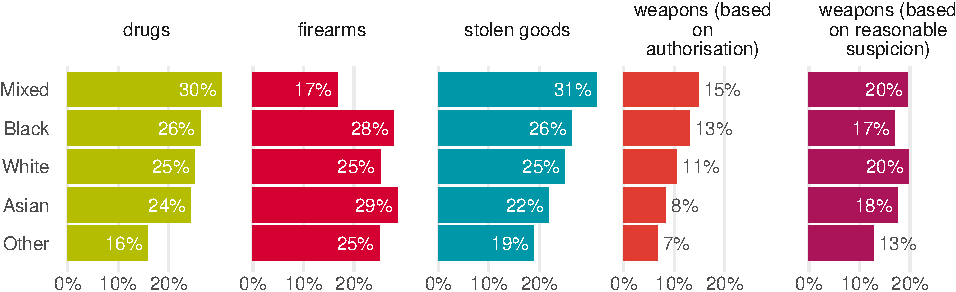
\includegraphics{2020-Q3_files/figure-latex/chart-outcomes-ethnicity-1} 

}

\caption{Proportion of searches resulting in a formal outcome, April to September 2020}\label{fig:chart-outcomes-ethnicity}
\end{figure}

\hypertarget{where-do-stops-happen}{%
\section{Where do stops happen?}\label{where-do-stops-happen}}

Stop and search is geographically concentrated in some parts of London: \textbf{half of searches between July and September 2020 occurred in 9\% of neighbourhoods}. Searches are also concentrated in deprived areas: 69\% of searches took place in neighbourhoods that were more deprived than average. In particular, 80\% of searches for weapons under section 60 occurred in the most-deprived half of neighbourhoods.

Of the 33 boroughs in London, the most searches in July to September 2020 took place in Westminster (4,550 searches), Newham (4,018) and Southwark (3,430), while the fewest took place in Richmond upon Thames (691 searches), Bexley (697) and Sutton (727). We can identify search hotspots by counting searches in each of about 2,000 equally-sized cells (Figure \ref{fig:chart-map}).

Of the 657 local-authority wards in London, the ward with the most searches between July and September 2020 was West End ward in Westminster, in which there were more searches than in 12 entire boroughs (Table \ref{tab:table-ward}).

Searches for weapons under section 60 can only take place in areas in which an inspector (a second-line supervisor) believes ``incidents involving serious violence may take place''. Of the 910 no-suspicion searches under section 60 from July to September 2020, more than half (54\%) took place in six boroughs. Meanwhile, there were no section-60 searches in 33 other boroughs.

\hypertarget{a-note-on-data}{%
\section{A note on data}\label{a-note-on-data}}

This report uses data published by the Home Office at \href{https://data.police.uk/}{data.police.uk} under the \href{https://www.nationalarchives.gov.uk/doc/open-government-licence/version/3/}{Open Government Licence version 3.0} for searches conducted by the Metropolitan Police Service or City of London Police, or by British Transport Police at a location in London.

Search rates are calculated using \href{https://data.london.gov.uk/dataset/ethnic-group-population-projections}{2020 estimates of the London population by age and ethnic group} produced by the Mayor of London. Rates based on residential populations are imperfect because some people being searched in London will live outside London, but the vast majority of people searched in London are likely to also live in the region. All ethnicity figures in this report are self-defined ethnicities.

This report is published under a \href{https://creativecommons.org/licenses/by/4.0/}{Creative Commons Attribution Licence version 4.0}, meaning you are free to copy or redistribute this material in any medium or format, and to remix, transform, and build upon this material for any purpose, even commercially, as long as you comply with the licence terms.

Thank you to Ben Bradford, Gavin Hales and Paul Quinton for comments on drafts of this report. Cover photo by \href{https://unsplash.com/photos/tvPvROBv0F4}{James Padolsey on Unsplash.com}

\newgeometry{top = 2cm, inner = 1cm, bottom = 3cm, outer = 1cm}



\begin{figure}[tb]

{\centering 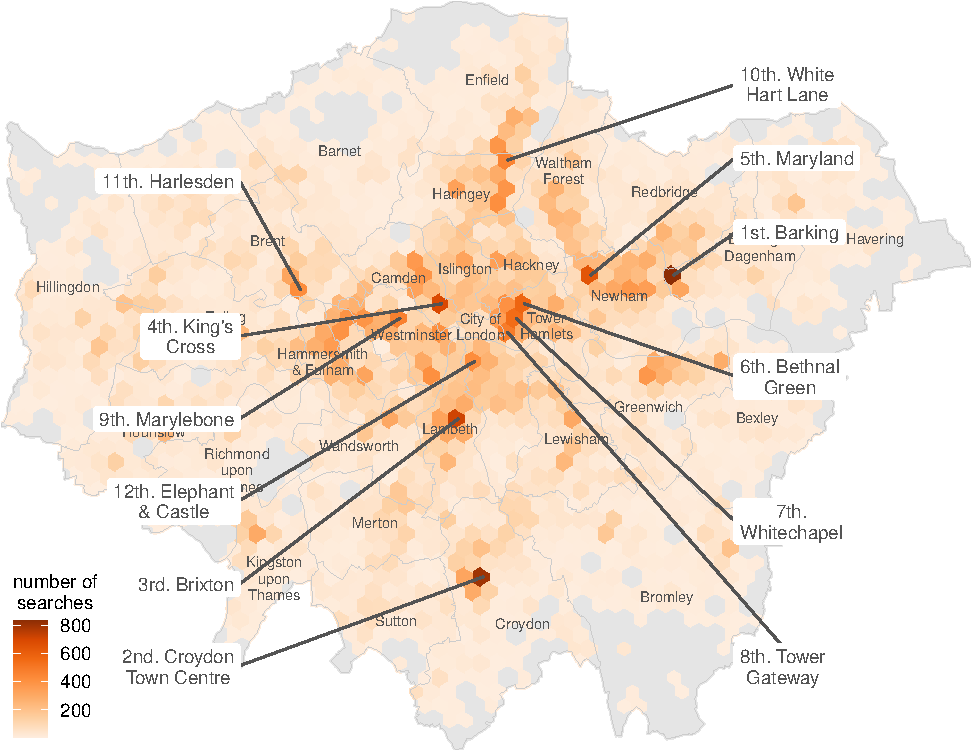
\includegraphics[width=19cm]{2020-Q3_files/figure-latex/chart-map-1} 

}

\caption{Location of searches, July to September 2020}\label{fig:chart-map}
\end{figure}

\begin{table}

\caption{\label{tab:table-ward}Local authority wards with the highest number of searches, July to September 2020}
\centering
\begin{tabular}[t]{lr}
\toprule
council ward & searches\\
\midrule
1. West End ward, Westminster & 1,196\\
2. St James's ward, Westminster & 848\\
3. Stratford and New Town ward, Newham & 709\\
4. Broad Green ward, Croydon & 669\\
5. Harlesden ward, Brent & 597\\
6. London Bridge \& West Bermondsey ward, Southwark & 568\\
7. Abbey ward, Barking and Dagenham & 530\\
8. Fairfield ward, Croydon & 503\\
9. Whitechapel ward, Tower Hamlets & 485\\
10. North Walworth ward, Southwark & 465\\
11. East Ham Central ward, Newham & 434\\
12. Woolwich Riverside ward, Greenwich & 430\\
\bottomrule
\end{tabular}
\end{table}

\restoregeometry

\end{document}
